\chapter{Interfaces}

\section{Connectors}

See \textbf{Fig. \ref{fig:connectors}} for details.

\begin{figure}[htbp]
    \begin{center}
    \includegraphics[width=4.9in]{images/502_connectors.png}
    \caption{Connectors.}
    \label{fig:connectors}
    \end{center}
    \end{figure}

\subsection{Power}

Power is connected via Connector J1 (Backpane Connector).

\begin{verbatim}
    J1 pin 24 -9V (is this used ???)
    J1 pin 25/26 +5V
    J1 pin 27/28 Gnd
\end{verbatim}

The specification calls for +5v and -9v, however, -9v is only required for the RS232 serial port (TXD, TXCLK and RTS). Not supplying -9v and connecting the -9v rail to ground replicates the circuit used in later machines such as the Superboard II and Compukit UK101. The simplest way to achieve this is to replace C38 with a wire link. See \textbf{Fig. \ref{fig:c38}}.

\begin{figure}[htbp]
    \begin{center}
    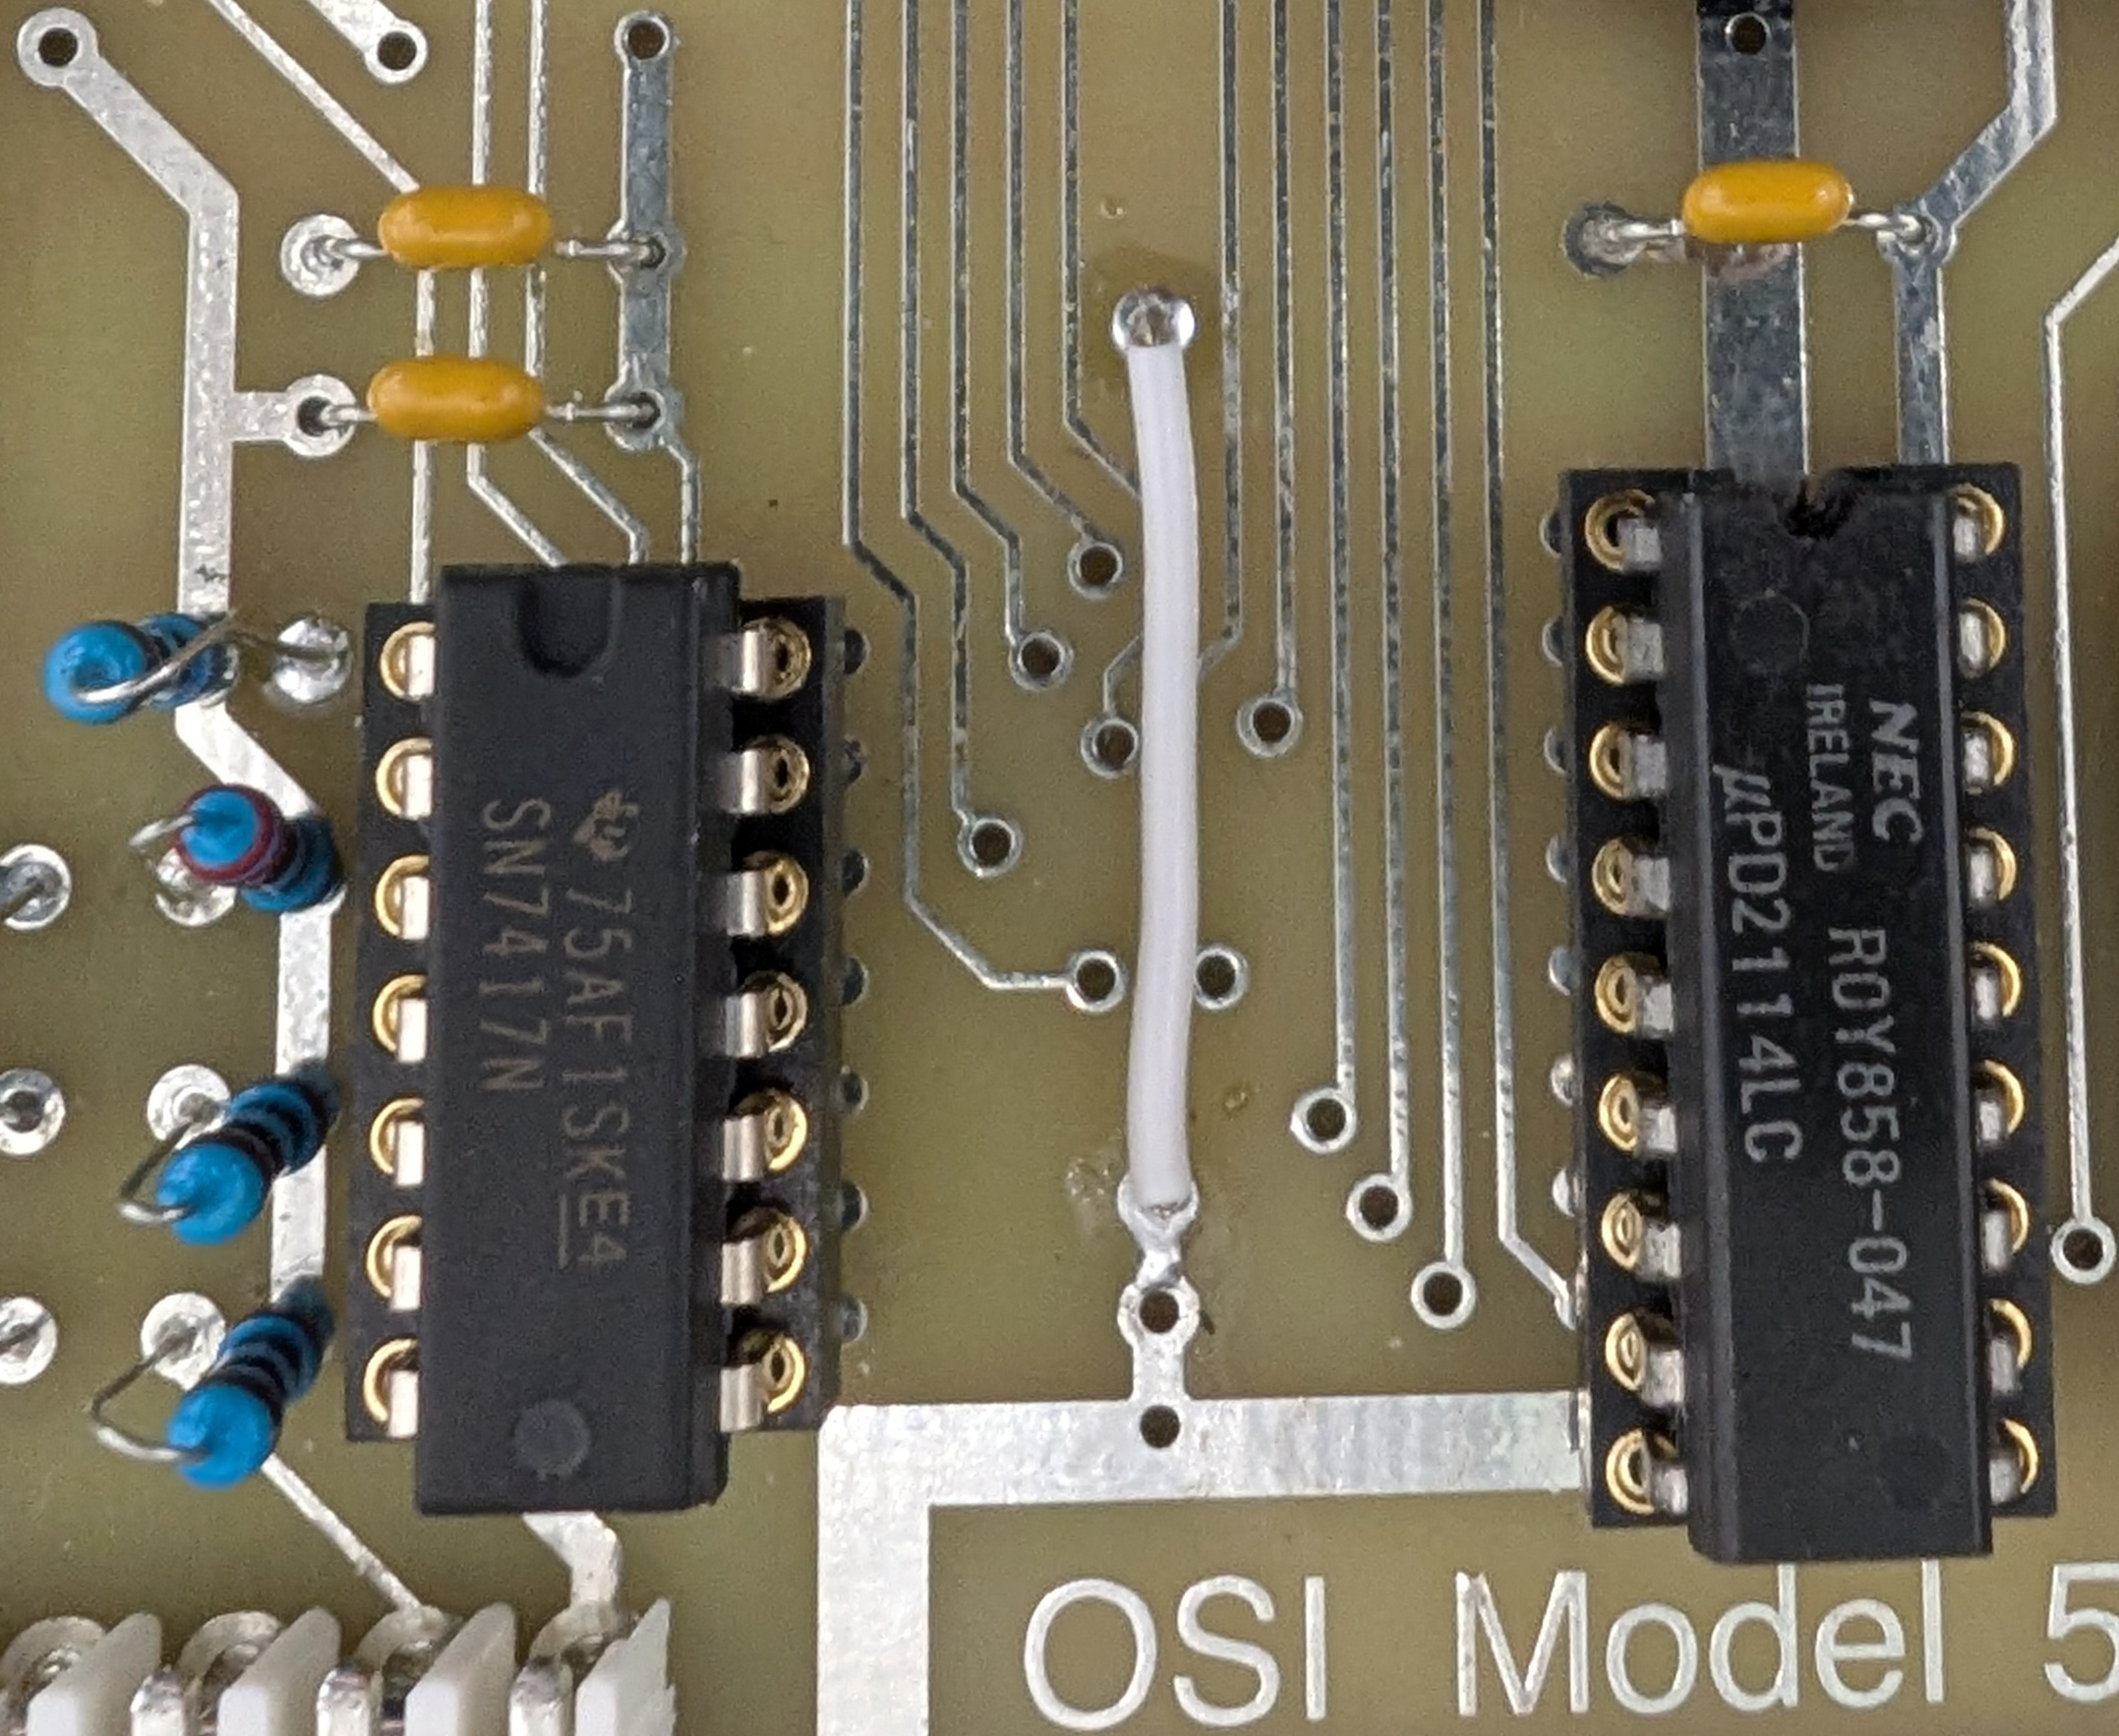
\includegraphics[width=4.9in]{images/C38.jpg}
    \caption{C38 replaced by a wire link.}
    \label{fig:c38}
    \end{center}
    \end{figure}

\subsection{Cassette Interface}

The Cassette Interface is available via connector J2 (with the backplane connector on the right, J2 is on the top).

\begin{verbatim}

    J2 pin 3 Reset
    J2 pin 8 cassette mic (output)
    J2 pin 9 Gnd
    J2 pin 11 cassette out (input) 

\end{verbatim}

\subsection{Serial Terminal} 

The serial terminal interface (RS232) is available via J3 (with the backplane connector on the right, J3 is on the bottom).

\begin{verbatim}

    J3 pin 1 RXD
    J3 pin 3 Receive Clock
    J3 pin 5 ACIA SP.I (see below)
    J3 pin 7 TXD
    J3 pin 9 Transmit Clock
    J3 pin 11 RTS

\end{verbatim}

Pin 5 of J3 is an input that can be configured via W3 to connect to the ACIA CTS or DCD inputs.

